\subsection{Graphene and hydrogen honeycomb lattice}
\label{subsection:graphene}
Our third example highlights the role of the high energy 
degrees of freedom not present in the low energy description 
but which are instrumental in renormalizing the effective interactions. 
We demonstrate this by considering the case of graphene, and by 
comparing it to artificially constructed counterparts without the high energy electrons. 

Although many electronic properties of graphene can be adequately 
described by a noninteracting tight-binding model of $\pi$ electrons~\cite{Castro2009}, 
electron-electron interactions are crucial for explaining 
a wide range of phenomena observed in experiments~\cite{Kotov2012}. 
In particular, electron screening from $\sigma$ bonding renormalizes 
the low energy plasmon frequency of the $\pi$ electrons~\cite{Zheng2016}. In fact, 
without the $\sigma$ electrons, a system of $\pi$ electrons with bare Coulomb interactions has been argued to be an 
insulator instead of a semimetal~\cite{DrutPRL2009, DrutPRB2009,  Smith2014, Zheng2016}. 

In order to probe this further, we disentangle the screening effect of $\sigma$ electrons from the bare interactions 
between $\pi$ electrons by considering a system of ``$\pi$-only" graphene. In this system, the 
$\sigma$ electrons are replaced with a static constant negative charge background. 
The role of $\sigma$ electrons is then clarified by comparing the effective model Hamiltonians of these two systems. 
We also study a honeycomb lattice of hydrogen atoms (with the same lattice constant $a=2.46$\AA~as graphene), 
which has a similar Dirac cone dispersion as graphene~\cite{Zheng2016}. 
%Thus, we expect the single body terms to be similar in all systems; the difference in their high energy structure 
%will manifest itself as differently renormalizated electron-electrons interactions. 

The low energy degrees of freedom correspond to the $\pi$ orbitals in graphene (and its $\pi$-only system) 
and $s$ orbitals in hydrogen (see Figure~\ref{fig:honeycomb_wan}). 
We consider a one-band Hubbard model. 
Due to the vanishing density of states at the Fermi level, the Coulomb interaction remains long-ranged, in contrast to usual 
metals where the formation of electron-hole pairs screens the interactions strongly~\cite{Zheng2016}. 
However, at least for certain aspects, the long ranged part can be considered as renormalizing the 
onsite Coulomb interaction $U$ at low energy \cite{Schuler2013, Changlani2015}. 
Therefore, we expect that one-band Hubbard model still remains a reasonable description of the low energy physics. 
\begin{figure}[hbt]
\centering
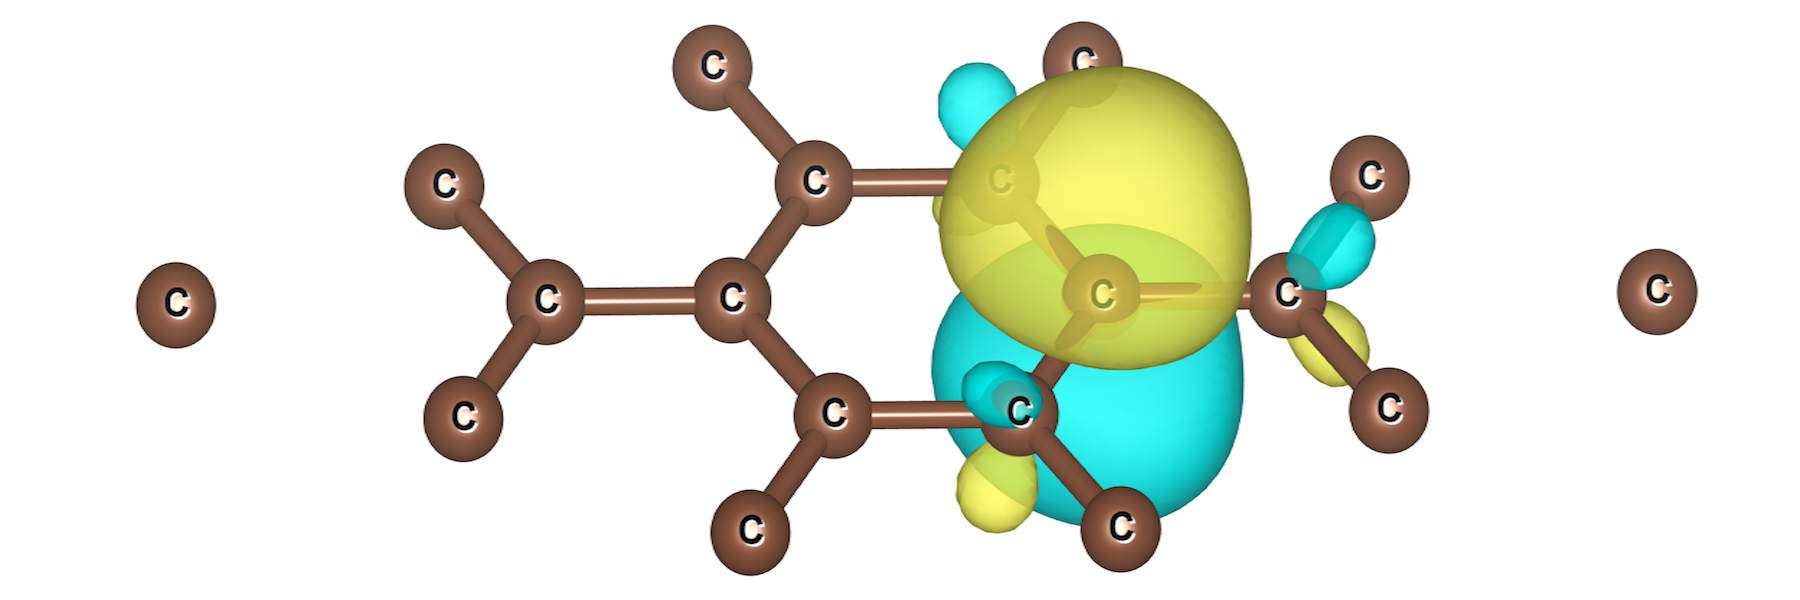
\includegraphics[width=0.40\textwidth]{./Figures/c_pi.png}
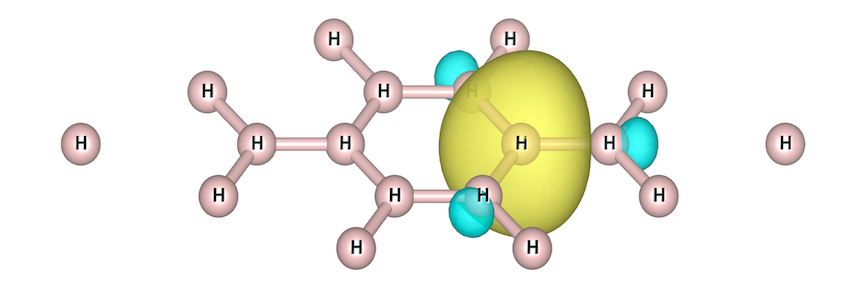
\includegraphics[width=0.40\textwidth]{./Figures/h_wan.png}
\caption{Wannier orbitals constructed from Kohn-Sham orbitals: (A) graphene $\pi$ orbital; (B) hydrogen $s$ orbital. }
\label{fig:honeycomb_wan}
\end{figure}

To estimate the Hubbard parameters, we used the DMD method using a set of 50 Slater-Jastrow wavefunctions that correspond 
to the electron-hole excitations within the $\pi$ channel (or $s$ channel for hydrogen system). In particular, for graphene, 
the Slater-Jastrow wave functions are constructed from occupied $\sigma$ bands and occupied $\pi$ bands, whereas for ``$\pi$-only" graphene, 
Slater-Jastrow wavefunctions constructed from occupied $\pi$ Kohn-Sham orbitals of graphene. The \textit{ab initio} simulations 
were performed on a $3\times3$ cell (32 carbons or hydrogens) and the energy and RDMs of these wavefunctions were
evaluated with VMC. \footnote{We expect further renormalizations in the corresponding DMC calculations~\cite{Changlani2015}, 
but we do not explore that aspect here} The error bars on our downfolded parameters are estimated using the Jackknife method. 
The results from our calculations are summarized in %Table~\ref{tab:grpheffm} 
Figure~\ref{fig:ne_aidmd_gh}.% shows the quality of the fits for the three systems.

%\begin{table}[ht]
%\centering
%\caption{Downfolding parameters for graphene and hydrogen.}
%\begin{tabular}{|c|c|c|c|}
%\hline
%Parameters [eV] & $\;\;\;\;$ graphene $\;\;\;$ & $\pi$-only graphene & $\;\;\;$hydrogen$\;\;\;$ \\
%\hline
%\hline
%$t$ & 3.61(1) & 2.99(1) & 3.73(1)\\
%$U$ & 7.16(3) & 14.8(2) & 9.47(5)\\
%\hline
%\end{tabular}

%\label{tab:grpheffm}
%\end{table} 

\begin{figure*}
\centering
  \begin{tabular}{@{}p{0.95\linewidth}@{\quad}p{\linewidth}@{}}
    \subfigimg[clip, width=0.325\linewidth]{(A)}{./Figures/grp_all_tu.pdf}
    \subfigimg[clip, width=0.325\linewidth]{(B)}{./Figures/grp_pi_tu.pdf}
    \subfigimg[clip, width=0.325\linewidth]{(C)}{./Figures/h_tu.pdf}
    \end{tabular}
\caption{Comparison of \textit{ab initio} (x-axis) and fitted energies (y-axis) of the 3$\times$3 periodic unit cell of graphene and hydrogen lattice: (A) graphene; (B) $\pi$-only graphene; (C) hydrogen lattice.}\label{fig:ne_aidmd_gh}
\end{figure*}


We find that the one-band Hubbard model describes graphene and hydrogen very well, as is seen from the small 
root mean square error of the predicted energies (shown in Figure~\ref{fig:ne_aidmd_gh}). The ratio of $U/t$ is smaller 
than the semi-metal-insulator transition critical value (3.8, for the honeycomb lattice \cite{Sorella2012}) in both graphene and hydrogen, 
which is consistent with both systems being semimetals. The two systems indeed have similar hopping constant $t$, 
consistent with the fact that they have similar Fermi velocities at the Dirac point. However, 
the difference in their high energy structure manifests itself as different renormalizated electron-electrons interactions, 
explaining the difference in $U$. 

Most prominently, the ``$\pi$-only" system has much larger $U/t$ ($\sim4.9$) compared to graphene, which is large enough 
to push it into the insulating (antiferromagnetic) phase. %of the honeycomb lattice Hubbard model. 
Another important difference, which matches with our physical intuition, is that graphene has larger $t$ than $\pi$-only graphene. 
This is attributed to the $\sigma$ electrons pushing $\pi$ electrons away from the ions through exchange-correlation interactions, 
which makes it easier for the $\pi$ electrons to hop to nearby sites. 

Thus, downfolding shows the clear significance of $\sigma$ electrons in renormalizing the effective onsite interactions of the $\pi$ orbitals. 
The $\sigma$ electrons change \textit{both} $t$ and $U$, making graphene a weakly interacting semimetal instead of an insulator.
%In summary, we have demonstrated that the effective models constructed using this approach effectively reflect the renormalization/screening effect from high energy degree of freedom, and correctly characterize the low energy dynamics of the system. 
